\section{Methodology}\label{sec-methodology}
The use of ICT virtual resources and digital tools in ESP classes during
wartime has been studied through analysis of scientific and
methodological literature. This has allowed for the development of an
educational technology that can be implemented at all stages of the
learning process. Both in preparation for classes and during the
learning process, the specified technology can be used for explaining
new material, fixing errors, repeating information, checking for
understanding, correcting mistakes, and summarizing learning material.
This approach allows for the principles of activity, interactivity, and
a dialogic style of education to be employed, while also combining
individual and group work. Additionally, it helps to maintain students'
psychological comfort, optimize the process of ESP learning, and develop
students' POECC. The ICT tools presented can be used to engage and
motivate students in online classes, diversify visual aids, and create
interactive educational materials for whiteboards. Despite the
challenges of wartime and remote learning, resources such as Skype,
Blogger, Teams, and Zoom enable the organization of individual group
work, communication with students, creation of various tasks, and
automatic evaluation of their completion. The described platforms have
several advantages, including the ability to use free versions,
accessibility from different browsers and devices, and an
easy-to-understand interface that demonstrates the
tool\textquotesingle s capabilities. A\textbf{ }variety of content and
formats, including tests, quizzes, puzzles, crosswords, games, mind
maps, and diagrams in Kahoot, Quizizz, Quizlet, Learning Apps can
help to prevent the monotonous repetition of typical exercises. Students
can create their own organizers and bookmarks using tools such as
Padlet, Evernote, and Pinterest. Effective visual aids for presenting
learning material include Canva, Prezi, Maze, and Row Toon. The online
platforms Dropbox, Padlet, Pinterest, and Penzu enable users to share
their work and ideas. Students do not always have access to a computer,
so using platforms via mobile phones allows them to complete
tasks anywhere and without special technical requirements.

\subsection{Criteria}\label{subsec-criteria}
According to the theoretical analysis of the development of the POECC in
the motivational, cognitive, operational, and creative spheres of the
pre-service teachers of mathematics identified the following criteria:
motivational, cognitive, operational, and creative. Due to the specified
criteria, the development of POECC was assessed during the pre- and
post-stages of the experimental training of using ICT technology in ESP
learning. Table 1 presents the main criterion characteristics and
indicators.

\begin{table}[!htpb]
%\renewcommand{\arraystretch}{1.5}
\centering
\caption{POECC development criteria \cite{dmitrenko2020autonomous}.}
\label{tab-01}
\begin{threeparttable}
\begin{tabular}{l p{5cm} p{7cm}} 
\toprule
\emph{Criterion} & \emph{Characteristics of the criterion} & \emph{Indicators of the criterion} \\
\midrule
Motivational & ensures involvement in professional activity. It represents the positive attitude toward pedagogical creativity, awareness of the importance of POECC, which is revealed in satisfaction with the teaching profession, a desire for self-education, and active participation in work. & the desire to acquire knowledge, and improve	ESP skills; awareness of personal meaning and significance of	professional self-improvement; formation and orientation of the need for	POECC, self-education, and professional development; formation of motives; interest in ESP, intercultural knowledge, and skills; motivational interest in the chosen specialty. \\

Cognitive & is defined as a system of acquired knowledge and skills including purpose, principles, content, methods, techniques, and organizational forms of educational activities. & the completeness, correctness, and quality of the application of theoretical knowledge; the ability to select, process, and systematize ESP information; experience in recognizing norms of professional expression; free use of the thesaurus of professional terms; understanding and producing English texts related to the specialty. \\

Operational & is the appropriate application of POECС; as well as the ability to manage the educational process and one's own development. & the initiative, organization, self-discipline, self-control, productivity, the level of POECC, the presence of professional thinking, and the ability of self-education, etc. \\

Creative & describes the level of creativity and personal qualities of pre-service mathematics teachers, as well as their ability to think creatively, develop, analyze, and assess their readiness for professional activities in English for Specific Purposes (ESP). & the	ability to structure the process of solving educational tasks, outline the stages; correlate methods with types of tasks; self-control and adjust further activities; compare expected and obtained results; correlate practical experience and theoretical information. \\
\bottomrule
\end{tabular}
\end{threeparttable}
\source{\cite{dmitrenko2020autonomous}.}
\end{table}

Based on the given criteria, the pre-service teachers of mathematics were classified into three levels of POECC development: low, medium, and high (\Cref{tab-01}).

	\begin{table}[!htpb]
	\centering
	\caption{POECC development criteria \cite{dmitrenko2020autonomous}.}
	\label{tab-02}
	\begin{threeparttable}
    \begin{tabular}{ l p{4cm} p{4cm} p{4cm}}
    \toprule
	\emph{Criterion/Level} & \emph{Low level} & \emph{Medium level} & \emph{High level} \\
	\midrule
	Motivational & The student may not fully appreciate the personal and
				social importance of professional activity in ESP. They may not feel a
				strong need for it and may even view it negatively. As a result, they
				may only engage in ESP professional activity when required and may not
				demonstrate long-term commitment or independence. & The student is aware
				of the importance of professional activity in ESP formation of
				professional qualities, and willingly participates in it, shows positive
				emotions, quite active and independent in solving typical tasks but
				often requires a teacher's help. & The student clearly expresses
				persistent interest in ESP professional activity, eagerly 
				participates in it, shows responsibility, strives for independence and
				leadership, and actively shows positive emotions. \\
				Cognitive & The student has a limited understanding of ESP, recalling
				only basic concepts from memory and often misunderstanding their
				essence. They possess some ideas about the structure and methods of ESP
				professional activity, but these are not fully developed. & The student
				demonstrates an understanding of the role of ESP professional activity
				and possesses the necessary knowledge to explain, retell, and provide
				specific examples. However, there are some inaccuracies in their
				application of this knowledge when performing typical tasks. & The
				student has a fairly fluent command of terminology, can give accurate
				definitions and characteristics of concepts, clearly distinguishes the
				activity stages, passes existing knowledge, and applies it in new
				conditions to perform atypical tasks. \\
				Operational & The student is partially aware of the content of ESP
				professional activity and its operational composition, begins to carry
				it out, can report on his / her actions but cannot organize his / her
				actions without outside help, and cooperates with others quite
				successfully. & The student consciously and independently performs
				previously learned ESP professional activity in a typical situation and
				knows how to identify the inconsistency of a new task and a learned way
				of acting. & The student performs ESP professional activities quite
				fluently, is aware of each step, critically evaluates his / her actions
				at all stages, and can change a well-known method of action or build a
				new one to perform a non-typical task. \\
				Creative & The student uses the semi-patterned activity and the
				primitive tools, stays within the given or initially found method of
				action, and does not see alternative ways of performing the task. & The
				student looks for alternative solutions in a typical situation,
				independently combines known methods, analyses the task conditions, and
				is ready to describe the cause of difficulties or a new method. & The
				student freely applies acquired knowledge and a method of activity in
				non-standard situations, offers alternative ways of solving tasks, and
				reasonably chooses the optimal one. \\
				\bottomrule
            \end{tabular}
		\end{threeparttable}
		\source{\cite{dmitrenko2020autonomous}.}
	\end{table}

In the process of implementing developed technology, virtual resources,
and digital tools were used in the experimental ESP online training of
pre-service teachers of mathematics.

In order to provide free access, a resource center of teaching materials
intended for use by students was created. It was placed on a separate
page of the teacher's website \enquote{English for Students of Mathematics}.
The site page contained placement tests, current and intermediate
control tests; thematic texts, speech and language exercises; texts on
specialty for annotation and summary; an electronic manual; additional
materials: an English-Ukrainian mathematical dictionary, examples of
reading mathematical expressions, tips for writing annotations and
summaries, tips for choosing and using learning and communication
strategies, etc. (\Cref{fig-01}).

\begin{figure}[htpb]
\centering
\begin{minipage}{.65\textwidth}
\caption{Website page of ESP for pre-service teachers of mathematics.}	
\label{fig-01}
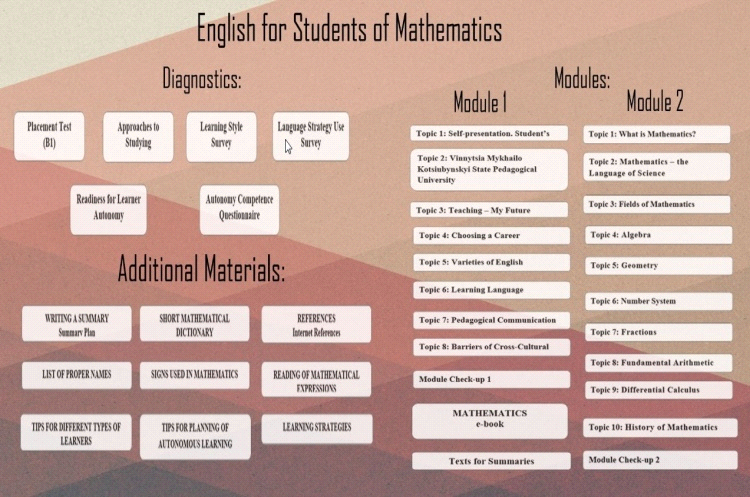
\includegraphics[width=\textwidth]{figure01}
\source{\cite{dmitrenko2020autonomous}.}
\end{minipage}
\end{figure}
The created e-textbook allowed the students to \begin{enumerate*}[label=\arabic*)]
	
	\item practice professional
	lexical skills; 
	\item carry out current control of the understanding of the
	content of the text on the specialty; 
	\item communicate using the learnt
	professional vocabulary; 
	\item discuss educational and professional problem
	situations; 
	\item prepare public speeches on a number of professional
	issues; 
	\item search for new textual, graphic and audio professionally
	oriented English information and analyze it; 
	\item write professional
        letters and documents in English (\Cref{fig-02}).
\end{enumerate*}

\begin{figure}[htpb]
\centering
\begin{minipage}{.65\textwidth}
\caption{Screenshot of the page (listening to the dialogue) of the e-textbook \enquote{Mathematics}.}	
\label{fig-02}
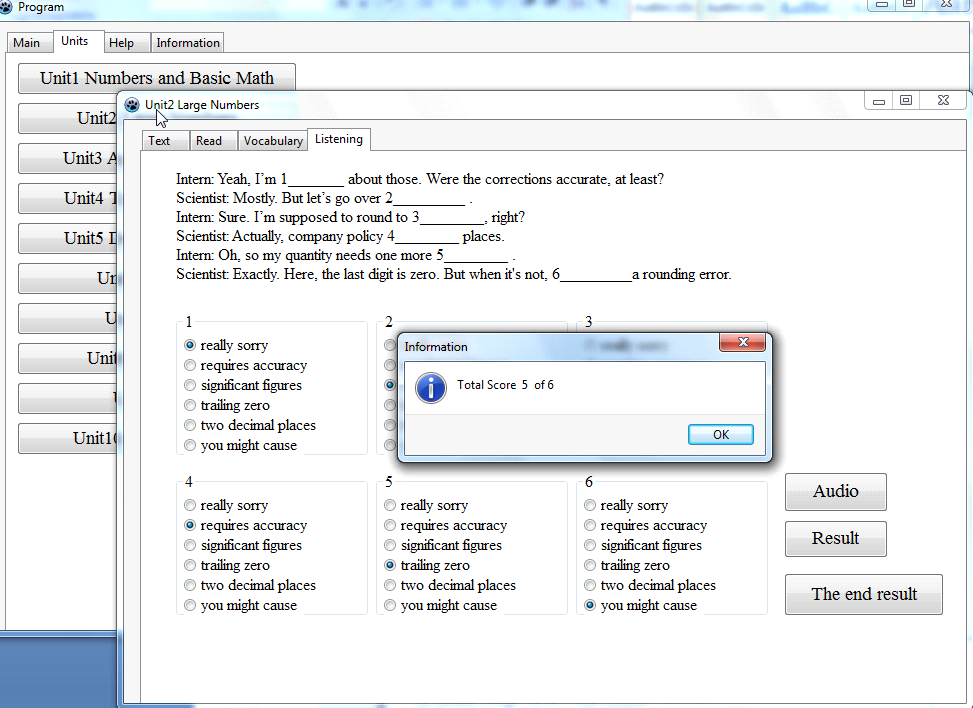
\includegraphics[width=\textwidth]{figure02}
\source{\cite{dmitrenko2020autonomous}.}
\end{minipage}
\end{figure}

Various applications have been used for interactive online ESP classes.
For example, the universal designer of interactive tasks
LearningApps.org was used to support the ESP learning process with the
help of interactive modules. Both the teacher and the student could
create interactive tasks based on ready-made templates. Such
verification and consolidation of the students' knowledge in a playful
way contributed to the formation of their cognitive interest in the ESP
educational component. The service included a gallery of publicly
available interactive tasks in English and all learning materials might
be posted publicly or for private use. An effective mobile web-based
learning application for ESP classes Quizlet was used to study and
repeat lexical and grammatical material with the help of self-made
flashcards, which contributed to the rapid assimilation of English
training material. The Quizlet Live application allowed students to
check the quality of the learned lexical material in an individual or
group format. The Kahoot!, was used to create tests, games, and quizzes
and is freely accessible from any browser on any device with internet
access. The teacher could create (or use a database of ready-made ones)
interactive tests, lead discussions, and present other learning
materials. Some examples of applications for creating exercises are
presented below.

\textbf{Example 1}. The purpose of the exercise is to acquaint students with the
typical features of using computers, to check the level of understanding
of the text, and to read silently (intensive reading). Instructions:
\enquote{Follow the link. Read the first paragraph of the text and write the
title. Check the correct answer by clicking on the button \enquote{Check
your answer}. Click on the arrow and move to another paragraph. You
have 15 minutes to do this} (\Cref{fig-03}).

\begin{figure}[htpb]
\centering
\begin{minipage}{.65\textwidth}
\caption{An example of an exercise in the application Learning Apps.}	
\label{fig-03}
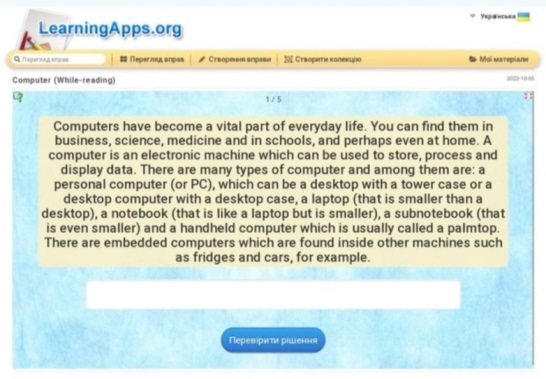
\includegraphics[width=\textwidth]{figure03}
\source{\cite{dmitrenko2020autonomous}.}
\end{minipage}
\end{figure}

\textbf{Example 2}. The exercise aims to check the level of understanding of
lexical items from the text. Instructions: \enquote{Follow the link. Match the
word with its definition. While doing the task, you will see the timer
which will count the time you have to complete the exercise. If you
choose the wrong answer, the time will be doubled. The person who
completes the task the fastest gets the highest score} (\Cref{fig-04}).

\begin{figure}[htpb]
\centering
\begin{minipage}{.65\textwidth}
\caption{A sample of an exercise in the Quizzlet application.}	
\label{fig-04}
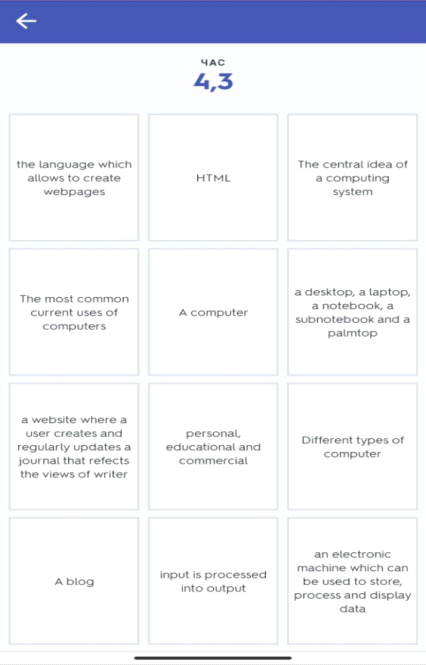
\includegraphics[width=\textwidth]{figure04}
\source{\cite{dmitrenko2020autonomous}.}
\end{minipage}
\end{figure}

\textbf{Example 3}. The purpose of the exercise is to check the level of reading
comprehension and text analysis. Instructions: \enquote{Take your mobile
phone and follow the link (\url{https://kahoot.it/}). Ask your teacher
for the code, enter it and your name. On the teacher's screen, you will
see the fact about computers and two sentences with red and blue colors.
Read the fact and choose the right color for yourself on the phone. If
you already know the fact, then you are doing great. If you don't know
the fact, then explain what exactly you want to discover about it. The
one who shares the opinion the most of all will get the highest score}
(\Cref{fig-05}).


\begin{figure}[htpb]
\centering
\begin{minipage}{.65\textwidth}
\caption{An example of an exercise in Kahoot!}	
\label{fig-05}
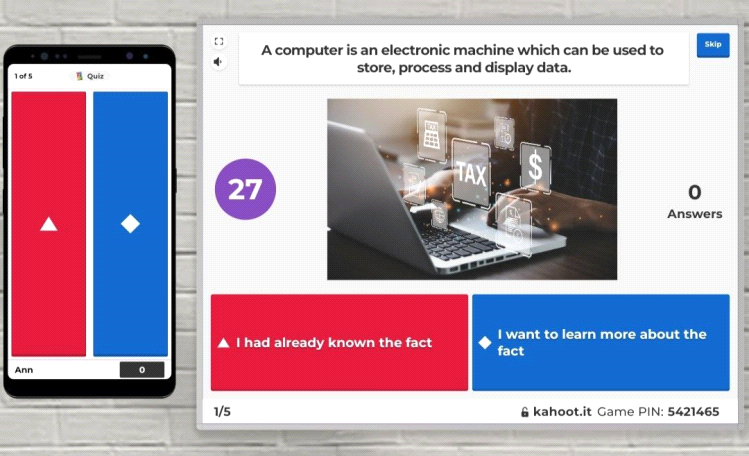
\includegraphics[width=\textwidth]{figure05}
\source{\cite{dmitrenko2020autonomous}.}
\end{minipage}
\end{figure}

\subsubsection{Participants}\label{subsubsec-participants}

The pre-service teachers of mathematics were divided into two
homogeneous groups: the control group (CG) – the formation of POACC
under usual conditions and the experimental group (EG) – the formation
of POACC under the influence of an active pedagogical factor – with the
use of virtual resources and digit tools. The participants of the study
were second-year students of the specialisation \enquote{Secondary Education.
Mathematics}, and \enquote{Mathematics} at the Faculty of Mathematics,
Physics and Computer Sciences, Vinnytsia Mykhailo Kotsiubynskyi State
Pedagogical University. The total number of participants was 100
students, 50 participants in CG and EG respectively. The experimental
training was carried out during one semester (17 weeks), and the ESP
classes were held twice a week. The ESP classes were held synchronously
online and lasted 80 minutes. Students were informed about the goals,
tasks, and conditions of experimental training and participated
voluntarily.

\subsubsection{The Study Stages}\label{subsubsec-thestudystages}

The study on the appropriateness of using ICT technology in ESP learning
by pre-service teachers of mathematics consisted of three stages. The
task of the \emph{first} stage was to measure the level of development
of the POECC of pre-service teachers of mathematics in EG and CG at the
beginning of the experimental training. The task of the \emph{second}
stage was to carry out the actual experimental training of ESP in EG
using the developed technology of ICT with virtual resources and digital
tools, and traditional training (without ICT tools) in CG. The task of
the \emph{third} stage was to diagnose and compare the level of
development of POECC of pre-service teachers of mathematics in CG and EG
after the introduction of an active pedagogical influence factor,
namely, the educational technology of using ICT in ESP learning.

\subsubsection{Instruments}\label{subsubsec-instruments}

The students' level of POECC was measured at the beginning and after the
experimental training (pre- and post-phases). The test was administered
to the students to assess the development of POECC according to the
following learning outcomes, which included 4 parts: \begin{enumerate*}[label=\arabic*)]
\item  knowledge of
basic English professional terms; 
\item the ability to translate
professional texts; 
\item the ability to analyze the content of English
professional sources; 
\item the ability to listen and understand the oral
professional speech.
\end{enumerate*}

The evaluation was carried out by experts (English teachers) on a
100-point scale for four components: knowledge of basic English
professional terms, translation of professional texts, content analysis
of English professional sources, and the ability to listen to oral
professional speech. Each component was evaluated in terms of 25 points.
The maximum level of development of each component was estimated at a
maximum of 25 points; the possible minimum was 1 point. The total score
for all components determined the level of development of the POECC of
pre-service teachers of mathematics: a low level – from 4 to 40 points;
an average level – from 41 to 74 points; and a high level – from 75 to
100 points. The assessment was carried out according to the
methodological recommendations of a group of experts.

The initial part of the test assessed the participants' understanding of
fundamental mathematical terms in English. The task required the
translation of fifty English terms, with each correct answer being
awarded two points. The second part of the test evaluated the students'
ability to translate professional English texts from English into
Ukrainian. Students were given to read and translate an English
professional text on a mathematical topic. The third part of the test
assessed students' capacity to analyze professional English sources and
select the appropriate section for further detailed study, analysis, and
use in pedagogical practice. The fourth part of the test evaluated
students' ability to comprehend spoken English in a professional
context. They were required to listen to a professional English text and
translate it into Ukrainian.

To assess group homogeneity and result reliability, we performed
statistical processing on the data using Pearson\textquotesingle s test.
We calculated the empirical value using the formula:

\vspace{2pt}
 
 
{\begin{center}
\large$X^{2}_{emp} = N . M . \sum_{i=1}^{L}\frac{ (\frac{n_{i}}{N}-\frac{m_{i}}{M})^{2}}{n_{i}+m_{i}} \label{formula-01}$
\end{center}}


\vspace{2pt}

\begin{itemize}
    \item N and M represent the numbers of EG and CG members respectively.
    \item The i-th level of pre-service teachers' readiness for ESP online
learning was demonstrated by the number of EG and CG members.
    \item The variable L represents the quantity of chosen levels. 
    \item The data was processed using the Microsoft Excel 2019 program.
\end{itemize}
